\documentclass{article}

\usepackage{amsmath}
\usepackage{amsthm}
\usepackage{amssymb}
\usepackage{float}
\usepackage{graphicx}
\usepackage[utf8]{inputenc}
\usepackage[english]{babel}

\newtheorem{theorem}{Theorem}

\title{%
	Machine Learning: Collectives of local decision makers\\
	\large Construction Of A Boundary Hunter
}
\author{Daniel Braithwaite}

\begin{document}

\maketitle

The goal of this project is to create neurons which insted of searching for a global minumum they will choose a specific part of the data to place their hyperplane. Consider the folowing situation in $\mathbb{R}^2$ where we have data split into two classes and the second class is boxed into a chevron shape. A single perceptron will go and place a horizonal line through the plane however this isnt telling us anything interesting. Prehaps something better to do is to align its self to one of the sides of the chevron, then if we added another "boundary hunter" it could align its self to the other side of the chevron.

\section{Simplified Situation}
Before worrying about this in the general case we aim to get a better understanding of the problem by first trying to solve the case described above. We first make some changes to how we have paramaterised our perceptron. We want to find a way which peforms the same as a standard perceptron before we start making it into a boundary hunter

\subsection{Point \& Gradient Paramaterisation}
We are trying to optimise a point (x,y) and a gradient. This is an alternative way to paramaterise our line. We are using sum squared error for our loss function and sigmoid as our activation. Each "boundary hunter" (BH) has the folowing weights vector $W = [m, x_0, y_0]$ and we consider two inputs to our BH, x and y. Our perceptron computes $z = (y - y_0) - m(x - x_0)$ and then outputs $o = f(z) = \frac{1}{1+e^{-z}}$.

\subsubsection{Comparason To Perceptron}
If we use the same set of data to train both our standard perceptron and our modified perceptron we see that our modified dosnt quite peform as well as the standard version. For both models below they where trained for 50000 iterations of the training data.

\begin{figure}[H]
\centering
  \begin{minipage}[b]{0.4\textwidth}
    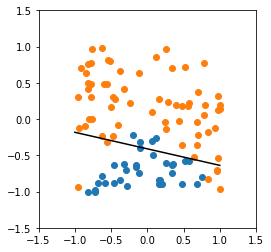
\includegraphics[width=\textwidth]{Standard-Perceptron.png}
    \caption{Standard Perceptron (SSE = 4.90)}
  \end{minipage}
  \hfill
  \begin{minipage}[b]{0.4\textwidth}
    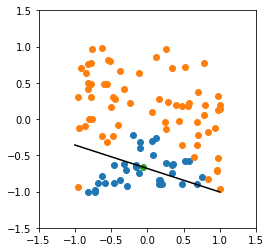
\includegraphics[width=\textwidth]{Modified-Perceptron-(Point-Grad).png}
    \caption{Modified Perceptron (SSE = 7.56)}
  \end{minipage}
\end{figure}

I propose that this way of constructing our perceptron is less powerful than the standard way. Consider when we are optimising our point-slope representation, 

\begin{align*}
y - y_0 &= m(x - x_0) \\
y &= y_0 + mx - mx_0 \\
y &= mx + (y_0 + mx_0)
\end{align*}

We have just shown that (as we would expect) we can convert out point-slope representation into a intercept-slope representation. From here we see we can convert into something that could be represented by our origonal perceptron.

\begin{align*}
y = mx + (y_0 + mx_0)\\
\Rightarrow -(y_0 + mx_0) -mx + y
\end{align*}

So given the generic form of our standard perceptron $A + Bx + Cy$ we see here that our modified perceptron can only ever learn a representation where C = 1, limiting what we can achieve. An easy way to check this is to see what happens if we use a standard perceptron to learn the data but keep the third weight (i.e. C) fixed at 1. Sure enough we get the folowing result when we run that experement over 50000 iterations.

\begin{figure}[H]
\centering
  \begin{minipage}[b]{0.4\textwidth}
    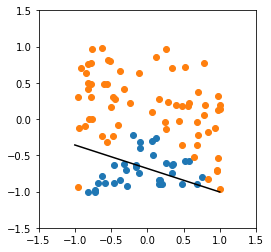
\includegraphics[width=\textwidth]{Standard-Perceptron-(C=1).png}
    \caption{Standard Perceptron with C = 1 (SSE = 7.56)}
  \end{minipage}
  \hfill
\end{figure}

So we are able to conclude that this method is unsuitable

\subsection{Normal \& Point Paramaterisation}
This method involves learning the normal vector (which is what the standard perceptron is doing) along with a point on the hyperplane. This increaes the number of paramaters we have to learn by n (when we are in $\mathbb{R}^n$ but this is necessary as to implement a BH we have to define some neighbourhood in which we care about and to do this we need to define it around some point on our hyperplane. So consider the folowing situation, we are learning the vector $n = [n_1, ..., n_n]$ normal to our hyperplane, the vector $a = [a_1, ..., a_n]$ which is on our hyperplane. We define $x = [x_1, ..., x_n]$ as our inputs making our weighted sum

\begin{align*}
z = \sum_{i=1}^n n_i * (a_i - x_i)
\end{align*}

We are still using SSE for loss and Sigmoid for actvation.

\subsubsection{Comparason To Perceptron}
Like before we compare the two paramaterisations using the same data and over 50000 iterations in the 2D case. In the graph for the modified perceptron the green point is our vector on the hyperplane.


\begin{figure}[H]
\centering
  \begin{minipage}[b]{0.4\textwidth}
    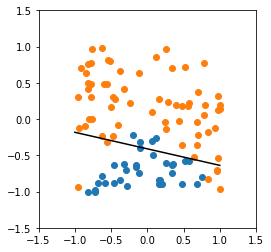
\includegraphics[width=\textwidth]{Standard-Perceptron.png}
    \caption{Standard Perceptron (SSE = 3.90)}
  \end{minipage}
  \hfill
  \begin{minipage}[b]{0.4\textwidth}
    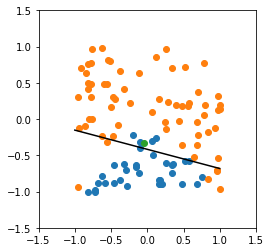
\includegraphics[width=\textwidth]{Modified-Perceptron-(Normal-Point).png}
    \caption{Modified Perceptron (SSE = 3.90)}
  \end{minipage}
\end{figure}

This modified perceptron has all the quallitys needed to proceid with creating the boundary hunters, whats better is this also generalizes to the $\mathbb{R}^n$ case.

\section{Boundary Hunter}
Using the \textbf{Normal \& Point Paramaterisation} from before we construct boundary hunters, first we have a simple case where the area of intererest for each boundary hunter is simpley a circle with fixed radius, our goal is to make this area of interest an ellipse which the BH will learn.

\subsection{Loss Function Design: Attempt 1}
We wish to convert our Perceptron into a Boundary Hunter so to begin we start with designing a suitible loss function. So firstly we want to have some notion of how responsible a boundary hunter is for a given data point, for now we will just denote the responsibility for data point n by $r_n$ and worry about calculating this later. Consider our boundary hunter as reducing the uncertuanty of the classes for each of the data points. As the datapoints get further away from our radius of expertees we become more uncertain about the class of the datapoint. So a reasonable loss function is 

\begin{align}
\frac{1}{n} \sum_{i=0}^n r_i(C_i log(y_i) + (1-C_i)log(1-y_i)) + (1-r_i) log(1/2)
\end{align}

But how do we construct $r_i$. We would like the folowing propertys of a responsibility function

\begin{enumerate}
\item Making the area of interest include all points will reduce loss to standard log loss.
\item All points inside the area of interest should have the same responsibility.
\item Responsibility for points outside the area of interest should decrease as distance from area increases.
\end{enumerate}

The folowing function seems like a good place to start. The responsiblity for any point inside the area of interest is 1, and as the data points get further away the responsiblity decreases

\begin{align}
r_i = 1 - \frac{max(0, d-r)}{abs(d-r) + 0.1}
\end{align}


\subsubsection{Experemental Results}
We train our boundary hunter over the same data for 10000 iterations and the result is somewhat uninteresting, it simply learns an area of interest which contains the entire data set, reducing our loss function to the standard cross entropy loss function 

\begin{figure}[H]
\centering
  \begin{minipage}[b]{0.4\textwidth}
    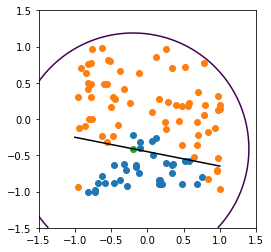
\includegraphics[width=\textwidth]{BoundaryHunter-Attempt1-01.png}
    \caption{Boundary Hunter with (1) as loss}
  \end{minipage}
  \hfill
\end{figure}

With corosponding line equation $y = -0.19877x -0.44949$. As demonstraited this line is almost identical to the one learned by a normal  \& point perceptron (descrepencies may be caused by longer training for standard perceptron). This demonstraites that this loss is not sutible

\subsubsection{Justification For Results}
So consider our loss for a given data point with target $t$, prediction $y$ and responsibility $r$. WILOG assume $t = 1$. So then we are left with $r\ log(y) + (1-r)\ log(\frac{1}{2})$. And $log(y) = log(\frac{1}{2})$ in the worst case. So we can always at least obtain an equivelent solution by setting $r = 1$ for each data point. Peforming such a thing is equivlent to including all points inside the area of interest.  

\subsubsection{Reflection}
Esentially we want to reward our boundary hunter if it is an expert in a given region, so if it gets things wrong outside its area of interest thats good, and if it gets things correct outside its area of interest then thats bad.

\subsection{Loss Funcction Design: Attempt 2}
Based on our previous findings a more in depth consideration of a suitable loss function is required. Consider the folowing properties of our ideal loss function. The basic idea is that we want to become experts in a given region
\begin{enumerate}
\item As a data point gets further away from our area of interest we "care less" about our accuracy for classifying that point.
\item Increasing area of interest should decrease the loss iff increasing the area of interest allows us to classify more points correctly.
\item Decreasing area of interest should decrease the loss iff reducing area of interest allows us to classify less points incorrectly in our area
\end{enumerate}

We can simplyfy these ideas into rules

\begin{enumerate}
\item We want to be as accurate as possible in our area of interest and care less about our accuracy based on how "responsible" we are for the data point.
\item We should be penalised for classifying things correctly out side our area of interest based on how "not responsible" we are for the data point (i.e. if we are classifying a data point correctly but it is just outside our area of interest then we should be penalised).
\item We should be rewarded for classifying things incorrectly our side our area of interest based on how "not responsible" we are for the data point (i.e. if we are classifying a data point incorrectly and its just outside our area of interest then we should be rewarded).
\end{enumerate}

We now wish to convert this into a loss function. Item (1) is refering to $r_n$ multiplyed by the standard cross entropy. But now by using (1) we are doing the oposite of (2) and (3). Item (2) and (3) refer to $r_n$ multiplyed by what we call the "inverted cross entropy", here we restrict the "inverted cross entropy" to just the points that are not inside our area of interest. Where the standard cross entropy really hates to get things wrong, the inverted cross entropy really hates to get things right. So we propose the folowing as our loss where $H(t, y) = t\ log(y) + (1-t)\ log(1-y)$ is our standard cross entropy and we define $H^-(t, y) = t\ log(1-y) + (1-t)\ log(y)$ as our "inverted cross entropy" giving us the folowing loss function

\begin{align}
- \big( \frac{1}{n} \big[ \sum_{i=0}^n H(t_i, y_i) \big] + \frac{1}{|O|} \big[ \sum_{i \in O} H^{-}(t_i, y_i) \big] \big)
\end{align}

Where $O$ is the set of points not in our area of interest.

\end{document}
